\section{WKB Continued}
\subsection{A review of WKB motivation and derivation}
The basic idea of WKB is the following. What we want to do is to find some approximation where we can study effects that cannot be revealed using perturbation theory. Many functions can be expanded in a series $\sum_n c_n g^n$, but not all effects can be computed; namely those that go as $e^{-\frac{1}{g}}$ (as all derivatives of these classes of functions vanish). So, we want to study a different type of approximation to PT which allows us to probe such functions.

Our WKB approximation tells us that the wavefunction has the approximate form:
\begin{equation}
    \psi(x) \sim e^{\pm i \int^x \frac{p(x')dx'}{\hbar}} \frac{1}{\sqrt{\abs{p(x)}}}
\end{equation}
The way we did our expansion is justified so long as:
\begin{equation}
    \dod{}{x}\left(\frac{\hbar}{p(x)}\right) \ll 1 \implies \left| \dod{\lambda}{x}\right| \ll 1
\end{equation}

\subsection{When does WKB hold?}
We take $p(x) = \sqrt{2m(E - U(x))}$ and so:
\begin{equation}
    \dod{}{x}\left(\frac{\hbar}{p(x)}\right) \ll 1 \implies \dod{}{x}\left(\frac{\hbar}{\sqrt{2m(E - U(x))}}\right) \ll 1
\end{equation}
so then:
\begin{equation}
    \left|\frac{\hbar}{\sqrt{2}m}\frac{1}{(E - U)^{3/2}}\frac{1}{2}\dod{U}{x}\right| \ll 1
\end{equation}
If $E \gg U$ then:
\begin{equation}
    \left|\frac{\hbar}{\sqrt{2}m}\frac{1}{E^{3/2}}\frac{1}{2}\dod{U}{x}\right| \ll 1
\end{equation}
So for excited enough states, this approximation is always justified (e.g. the Harmonic oscillator has $E \sim n$, so for $n$ sufficiently large the LHS is small). However, we also see places where the approximation is never justified; in particular, for $E \sim U$ (the turning points) the LHS explodes and so the condition is not satisfied.

Note we have been assuming $\od{U}{x} \sim 1$ throughout.

\subsection{A simple example}
We consider some smooth potential profile $U(x)$ in an infinite square well. 

\begin{figure}[htbp]
    \centering
    \begin{tikzpicture}[scale=1]
        \filldraw[color=gray!30, fill=gray!30] (0, 0) -- (-2, 0) -- (-2, 3.5) -- (0, 3.5) -- cycle;
        \filldraw[color=gray!30, fill=gray!30] (3, 0) -- (3, 3.5) -- (5, 3.5) -- (5, 0) -- cycle;
        \draw[latex-latex, thick] (-2, 0) -- (5, 0);
        \draw[-latex, thick] (0, 0) -- (0, 3.5);
        \draw[-latex, thick] (3, 0) -- (3, 3.5);
        \node[below] at (0, 0) {$x = 0$};
        \node[below] at (3, -0.1) {$x = a$};
        \node[above] at (-1, 1.75) {$U = \infty$};
        \node[above] at (4, 1.75) {$U = \infty$};
        \draw [thick] (0, 2) to [ curve through ={(0.25, 1.95) ..(0.5,1.75) .. (0.75, 1.65)   . . (1, 1.6) . . (1.5,1.375) . . (1.75, 1.5) ..  (2, 1.45) .. (2.5,1.65) .. (2.75, 1.75).. }] (3,2);
        \node[] at (1.5, 1.8) {$U(x)$};
    \end{tikzpicture}
    \caption{A smooth potential profile $U$ enclosed in a infinite square well. We will find applying WKB gives rise to the Bohr-Sommerfield quantization condition.}
    \label{fig-infinitesquarewellWKB}
\end{figure}

We have that:
\begin{equation}
    \psi_\pm (x) = e^{\pm i\phi(x)}
\end{equation}
where:
\begin{equation}
    \phi(x) = \int_0^x \frac{p(x')dx'}{\hbar}
\end{equation}
as usual:
\begin{equation}
    p^2 = 2m(E - U)
\end{equation}
taking a superposition of the solutions, we have:
\begin{equation}
    \Psi(x) = \psi_+(x) + \psi_-(x) = \frac{A_+}{\sqrt{p}}\cos(\phi(x)) + \frac{A_-}{\sqrt{p}}\sin(\phi(x))
\end{equation}
But by the boundary conditions, $\Psi(0) = 0$ and so since $\phi(0) = 0$ we find that $A_+ = 0$. Then, since we also have that $\Psi(a) = 0$ and so from $\sin(\phi(a)) = 0$ we find that $\phi(a) = n\pi$. Therefore:
\begin{equation}
    \int_0^a \frac{p(x')dx'}{\hbar} = \pi n
\end{equation}
Note in the special case where $U(x) = 0$, we can carry out the integral explicitly  and find:
\begin{equation}
    \frac{pa}{\hbar} = \pi n
\end{equation}
and solving for the energies:
\begin{equation}
    E_n = \frac{\hbar n^2\pi^2}{2ma^2}
\end{equation}
which is exactly the result we got from doing it analytically in our first QM class.

We can study the conditions for the validity of the WKB solutions in this case. As before, we have:

\begin{equation}
    \left|\frac{\hbar}{\sqrt{2}m}\frac{1}{(E - U)^{3/2}}\frac{1}{2}\dod{U}{x}\right| \ll 1
\end{equation}

So in the limit where $E \gg U$:

\begin{equation}
    \left|\frac{\hbar}{\sqrt{2}m}\frac{1}{E^{3/2}}\frac{1}{2}\dod{U}{x}\right| = \left|\sqrt{\frac{m}{\hbar}}\frac{1}{\pi^3n^3}\dod{U}{x}\right| \ll 11
\end{equation}

So for sufficiently large $n$ this holds (actually, in the case of $U = 0$ throughout the well the derivative vanishes everywhere so it holds even more generally, trivially).


\subsection{Connection Formulae - Motivation and Setup}
We now study the turning points; the setting is sketched in Fig. \ref{fig-connectionformula}.

\begin{figure}[htbp]
    \centering
    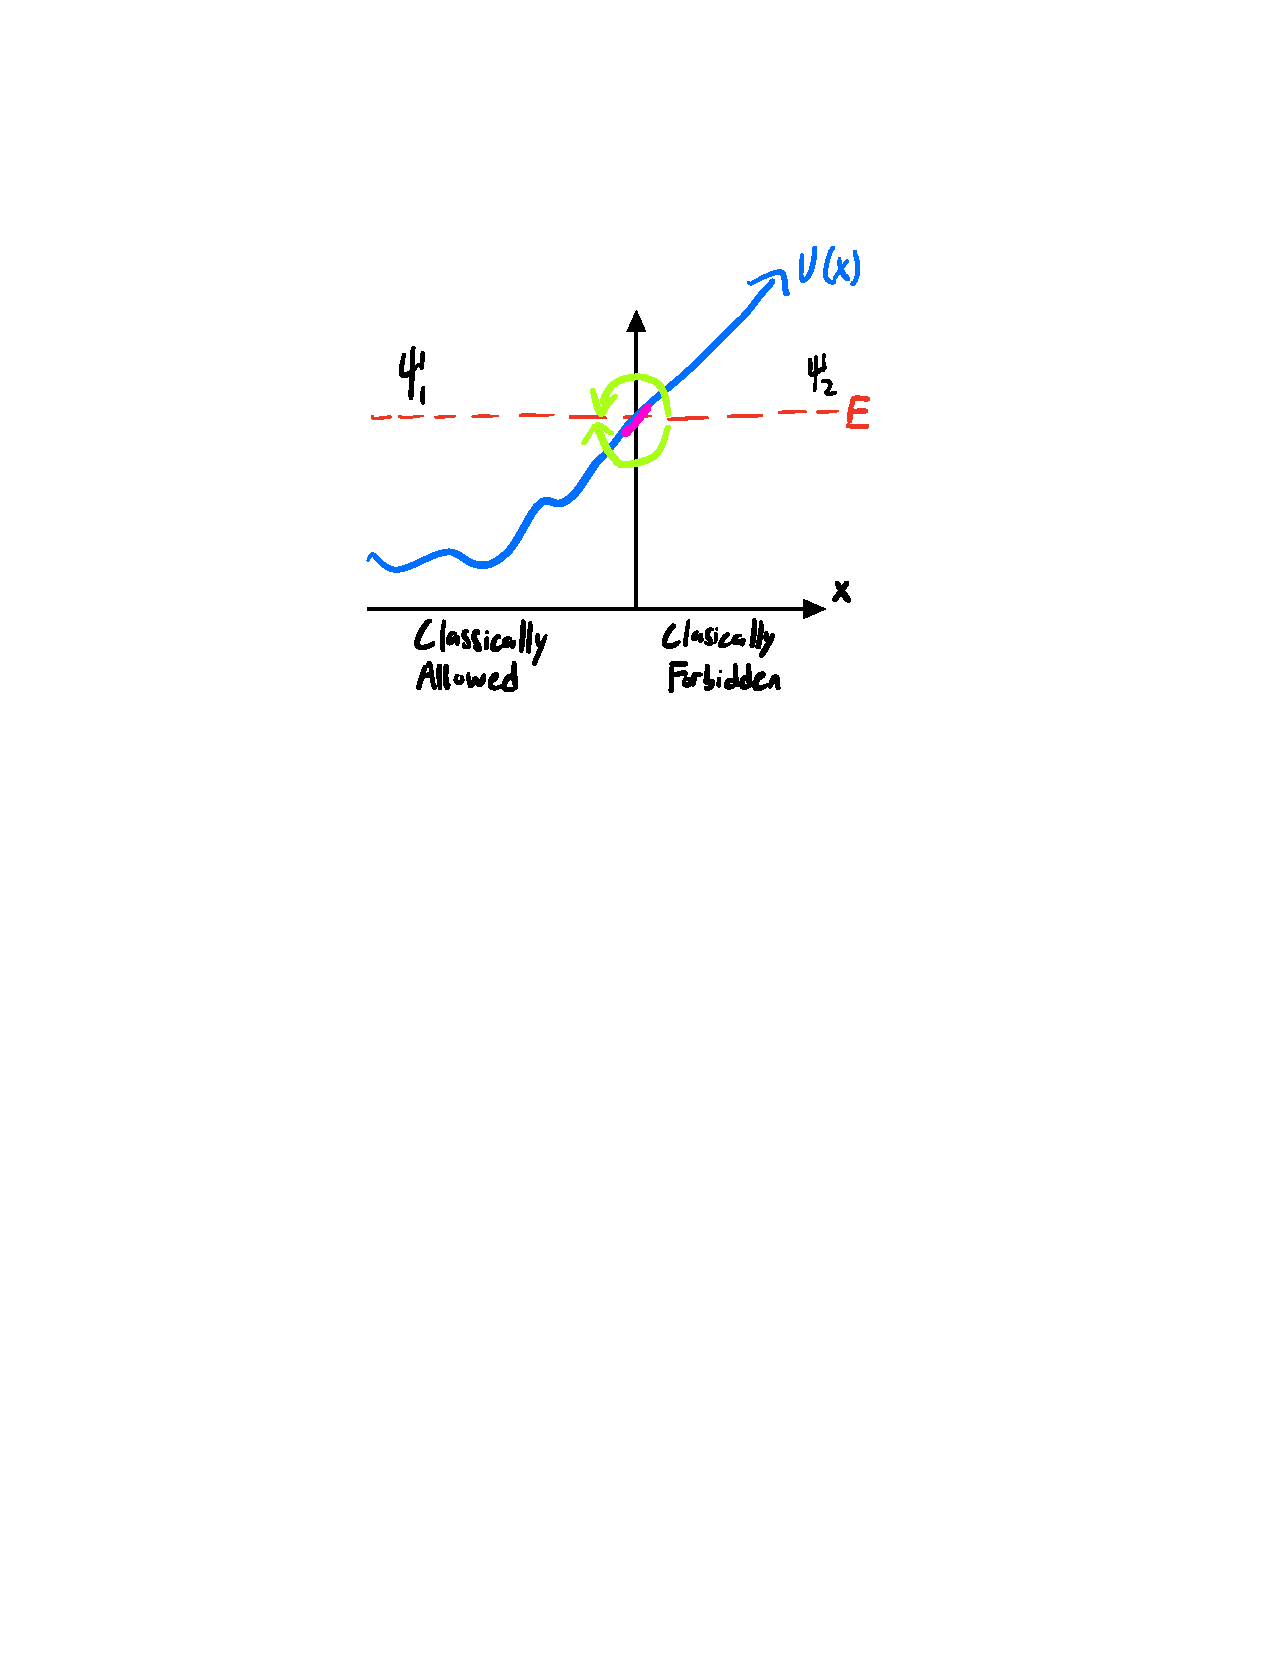
\includegraphics[scale=0.8]{Images/connectionformula.pdf}

    \caption{Determining the WKB solution at the turning points. On the left, we have the classically allowed ($E > U$) region for the particle, where the solutions $\psi_1$ are imaginary exponentials. On the right, we have the classically forbidden ($E < U$) region for the particle, where the solutions $\psi_2$ are decaying exponentials. We now need to determine what happens when $E \approx U$. The standard method is to consider the linear potential solutions of Airy functions at the turning point to piece the two together (pink). We consider a quicker argument, where we analytically continue the function in the complex plane by carrying out integrals from $0 \to \pi$ and $0 \to -\pi$ (green).}
    \label{fig-connectionformula}
\end{figure}


In the classically forbidden region (with $E < U(x)$) we can do exactly the same computations as we did for the classically allowed region; the only difference is now:
\begin{equation}
    \frac{p^2}{2m} = E - U(x)
\end{equation}
And so we obtain different WKB solutions:
\begin{equation}
    \frac{1}{\abs{p}}e^{\pm i \int^x \frac{p(x')dx'}{\hbar}} \to \frac{1}{\abs{p}}e^{\pm \int \frac{p(x')dx'}{\hbar}}
\end{equation}
where the left formula is for the classically allowed region, with $p^2/2m = E - U$ and the right formula is for the classically forbidden region with $p^2/2m = U - E$ (the exact same analysis from last class applies to study this region). In the classically forbidden region, we have:
\begin{equation}
    \psi_2(x) = \frac{D}{\sqrt{p}}e^{-\int_0^x \frac{p(x')dx'}{\hbar}}
\end{equation}
where $p^2 = 2m(U-E)$. Note that we \emph{only} consider the negative exponential solution; our wavefunctions must be normalizable and hence we throw away the $\sim \exp(+x)$ solution that is non-normalizable as $x \to \infty$.

So, we understand that far away from the turning point to the left (the classically allowed region) we have $e^{\pm i \int^x \frac{p(x')dx'}{\hbar}}$ solutions and far away from the turning point going to the right (the classically forbidden region) we have $e^{-\int_0^x \frac{p(x')dx'}{\hbar}}$ solutions. But what happens near the turning point? We discuss this now.

How do we do this? Many textbooks consider the linear potential near the turning point, which has known solutions of Airy functions. Far away to the left we find WKB sinusoidal solutions and far away to the right we have WKB exponential decay solutions. The Airy function is analytical and has the correct limits going away from the turning point. It is therefore a solution, and this is precisely what the connection formulae are. This is a very long derivation!

We go through this problem slightly differently. We recall that WKB does not apply at the turning point; our wavefunction is straightly wrong. We take $x \to z$ the complex plane. We then analytically continue our wavefunction, and obtain the connection formulae this way.

\subsection{Connection Formulae from Analytic Continuation}
We write down the superposition for $\psi_1$ (in the classically allowed region) in the following way. We have:
\begin{equation}
    \psi_1(x) = \left(\frac{B}{\sqrt{p(x)}}e^{+i\int_x^0 \frac{p(x')dx'}{\hbar}} + \frac{C}{\sqrt{p(x)}}e^{-i\int_x^0 \frac{p(x')dx'}{\hbar}}\right)
\end{equation}
We consider Taylor expanding the potential:
\begin{equation}
    U = U(0) + U'(0) x' = U_0 + U_0' x'
\end{equation}
such that now:
\begin{equation}
   \int  p(x)' dx' = \int x^{1/2}dx'\sqrt{2mU_0'}
\end{equation}
We now go to the complex plane. We write $x' = \rho e^{i\phi}$. We will do the integral and then do analytical continuation from $\phi = 0$ to $\phi = \pi$. Why can I do this? In the complex plane I can think that I can meander around the pole $E = U$ (compare to the real axis; we can't avoid the pole), so we don't hit it.

We carry out:
\begin{equation}
    \int_0^x \sqrt{x'}dx' = \frac{2}{3}\rho^{3/2}e^{i\frac{3}{2}\phi} = \begin{cases}
        \frac{2}{3}\rho^{3/2} & \phi = 0
        \\ \frac{2}{3}\rho^{3/2}e^{i\frac{3\pi}{2}} = -i\frac{2}{3}\rho^{3/2} & \phi = \pi
    \end{cases}
\end{equation}
We have thus ``collected the phase'' in the integral in the correct way. There is another term to consider; namely the $\frac{1}{\sqrt{p}}$. This collects a phase:
\begin{equation}
    \frac{1}{\sqrt{p}} \to \frac{1}{\sqrt{p}e^{i\pi/4}}
\end{equation}
When we analytically continue the classically forbidden region solution to the classically forbidden region, we obtian:
\begin{equation}
   \psi_2(x) = \frac{D}{\sqrt{p}}e^{-\int_0^x \frac{p(x')dx'}{\hbar}} \to \frac{D}{\sqrt{p}}e^{+i\int_x^0 \frac{p(x')dx'}{\hbar} - \frac{i\pi}{4}}
\end{equation}
For the other $e^{-i\ldots}$ term, we analytically contnue in the other direction, going from $\phi = 0$ to $\phi = -\pi$. So, we can write down $\psi_1$ as:
\begin{equation}
    \psi_1(x) = \frac{2D}{\sqrt{p}}\left(\cos(\int_x^0 \frac{p(x')dx'}{hbar} - \frac{\pi}{4})\right)
\end{equation}
where the cosine is obtained via the superposition of the two terms. We can write this equivalently as:
\begin{equation}
    \psi_1(x) = \frac{2D}{\sqrt{p}}\left(\sin(\int_x^0 \frac{p(x')dx'}{\hbar} + \frac{\pi}{4})\right)
\end{equation}
and the claim is the following: $\psi_2$ in classically forbidden region corresponds to this $\sin$, which is the superposition of the two plane waves in the classically allowed region, with the exact same coefficients.